\section{Electrical Power Subsystem}
\label{blDOEPS}

The electrical power system (EPS) is divided in to four parts: the power source, the energy storage, the power regulation and control and the power distribution. These are also the four main branches in the EPS design options structure. Each of these will be considered individually in this section. Figures \ref{pic_DOTeps_source}, \ref{pic_DOTeps_storage} and \ref{pic_DOTeps_reganddis} show the complete design option tree for the EPS.

\subsection{The power source}
\label{blDOsource}

Launch vehicles use primary batteries as power source because launches are quite short and thus can be kept fairly small. 
For missions lasting from weeks to years, however, batteries would be too large to be useful.
Typically, there are four types of power sources for longer missions: static power sources, dynamic power sources, fuel cells and photovoltaic solar cells.

Static power sources use a heat source for thermal-to-electric conversion. This conversion can be done by either a thermoelectric or a thermionic
concept. The thermoelectric converter uses the fact that the radioactive source (typically plutonium-238 or uranium-235) has a slow rate of decay.
Because of this, there exists a temperature gradient between the p-n junction of individual cells which is used to provide the desired direct current electrical output. The efficiency of such a system is about 5 tot 8\%.
Thermionic energy conversion, on the other hand, uses a hot electrode facing a cooler electrode to convert thermal energy to electrical.
These electrodes are sealed in a chamber containing an ionized gas. The hotter electrode can be seen as the emitter: it emits electrons that flow
across the inter-electrode gap towards the receiver (the cooler electrode). Once arrived, these electrons condense and return to the emitter through an electrical load connected externally between the two electrodes. Typical system efficiency is about 10 - 20\%.

Dynamic power sources function somewhat differently. They also use a heat source (typically concentrated solar radiation, radio isotopes or a nuclear-fission reaction) to produce thermal energy but the conversion method to electrical power is different. The generated heat is used to heat up a fluid to drive an energy-conversion heat engine. This is done using a Stirling cycle (efficiency of 25-30\%), a Rankine cycle (efficiency of 15-20\%) or a Brayton cycle (efficiency of 20-35\%).

Fuel cells are self-contained generators that convert the chemical energy of an oxidation into electrical power. They consist of two half-cells, each with an electrode and an electrolyte. The two half-cells may use the same electrolyte or they may use different ones.
In the fuel cell, one half-cell gets oxidized, it loses electrons, and the other is reduced, it gains electrons. As the electrons flow from
one half-cell to the other a difference in charge and thus an electric current is created. Fuel cells can be regenerative or not, unfortunately regenerative types have not been space-proven yet\cite{rees}.
The efficiency of fuel cells can be as high as 80\%, but will drop significantly at higher currents.

Photovoltaic solar cells are most common. They convert incident solar radiation directly in to electrical power. They consist of a semiconductor with metal plates on the top and bottom. Part of the incident solar radiation gets absorbed and is transferred to the
semiconductor. The energy excites electrons who are then free to move around. The metal plates move the electrons, which creates a current,
to power different subsystems. An efficiency of 29\% has been achieved \cite{doody1} in the lab, but production efficiencies are around 22\% \cite{larson}. Several options are available for the placing of the solar cells. The biggest difference is between solar panels and body-fixed solar cells. Body-fixed solar cells require a spinning satellite to be able to make optimal use of the cells. Solar panels, however, can be pointed towards the sun to have minimum cosine loss. The panels can be rigid or flexible, flexible panels being easier to transport but less strong than rigid panels.

A comparative table for the different power sources can be found in table 11-35 on page 410 of \cite{larson}.

\subsection{Power storage}
\label{blDOstorage}

Power storage is the second subdivision of the EPS. They can either provide all the power for short missions (primary batteries) or they provide back-up power for longer mission(secondary batteries).

Batteries can be both a power source and a power storage system. The following design options apply for both uses.

Primary batteries usually are used for short-term missions, up to about one day. Sometimes they are also used for long-term mission for tasks that require small power usage like memory back-up for example. They have a high specific energy density, which makes them a good choice for short missions. The number of batteries and their corresponding weight and size required for longer mission makes them a bad candidate. The most typical battery type use silver zinc, lithium thionyl chloride, lithium sulfur dioxide, lithium monoflouride and thermal cells.

Secondary batteries are mostly used on missions which use photovoltaics as a power source. Here they provide power when the solar panels are eclipsed and at moments when power requirement peaks. To keep the secondary batteries from becoming too large, they are required to be rechargeable. Some common secondary batteries are: Nickel-Cadmium, Nickel-Hydrogen (both space qualified), Lithium-Ion and Sodium-Sulfur (both under development). The nickel-hydrogen batteries have three space-qualified design variants: individual, common and single pressure vessel.

The individual pressure vessel contains only one electrochemical cell within. Usually they are connected in series to obtain the desired voltage.
The internal electrode stacks are connected in parallel.
The only difference between the individual and common pressure vessel is that the common pressure vessel has two electrode stacks, connected in series. This means that there are only half as much pressure vessel and less pieces, resulting in a higher specific energy density. 
Finally, the single pressure vessel has multiple cells connected in series that share a common supply of hydrogen. The cell stacks are each contained in a container with its own electrolyte supply\cite{larson}. 

Lithium-Ion batteries offer a significant advantage over nickel based ones. According to \cite{larson}, these types of batteries should be space qualified in the near future. At the moment, the effect of temperature on the performance is being researched. At the moment there are no components that are expected to be critically effected by temperature, resulting in a wide temperature range. Thus lithium-ion batteries may be a very interesting candidate for space applications in the near future\cite{lithium1}.

\subsection{Power regulation and control}
\label{blDOregulation}

The power regulation mainly concerns the bus regulation. The bus is the connection between power source and the different loads. It can be unregulated, quasi-regulated or fully regulated. The unregulated bus has its converters at the individual loads (see section \ref{blDOdistribution}).
A quasi-regulated bus has a battery charge regulator and a fully regulated bus also has a battery discharge regulator.
Batteries can be charged individually or in parallel. Batteries that are charged in parallel degrade faster. Because the current is not controlled, one battery could receive all the charge current. Eventually the batteries will balance out, but the battery life will be limited to about five years. To ensure a longer lifetime, they should be charged individually (for example by using a linear, charge-current-control design). A parallel charging system, however, is simpler and smaller than an individually charging system.

Because the optimum power source output and the bus input are different, a system has to be put in place to deal with this. An example of two possibilities will be given and explained for solar panels.
There are two ways of doing this: with a peak-power tracker (PPT) and with direct-energy-transfer (DET). 
A PPT is a non-dissipative system: it exacts the exact power the satellite requires (up to the arrays peak power). Every solar panel has a peak power point, which can be seen from the panels IV-curve. So the panel produces the most power at a certain current and voltage. But when a battery is charging, it is charged at it's own current and voltage. The result of this is that the battery will change the panel's current and voltage to it's own, forcing the solar panel to under perform. A PPT uses a DC/DC converter to change the solar panel's output to the required battery input, thus letting the panel perform at it's peak power point, increasing the efficiency. However, because the PPT is connected in series to the solar array, it uses about 4-7\% of the total power.

A DET system uses a shunt regulator to shunt away the excess power from the subsystem, usually at the array, to avoid internal energy dissipation. Shunt regulators can keep the bus voltage at a predetermined voltage. These systems are extremely efficient and has a lot of advantages over a PPT system: lower mass, less parts and a higher total efficiency at EOL.

\subsection{Power distribution}
\label{blDOdistribution}

A power distribution system (PDS) consists of the electrical load profile, the control options and fault protection.
After the load profile has been determined, the first choice to make is the type of current of the distribution system. Mostly direct current is used because spacecraft generate direct current. An AC/DC converter would need more electronics, resulting in more parts and a higher mass. 
But systems working with alternating current can be single phase or multiple phases\cite{kuphaldt}. THe main difference is that in a single phase system all voltages from the source vary in unison, whereas the different currents of the multi-phase system reach their peak value at different times. Each mode has its advantages and disadvantages. Single phase systems are simpler and thus cheaper but when higher loads are required multi-phase system are more useful. They can help to reduce vibrations, for example.

The PDS can either be centralized or decentralized. The decentralized option requires a converter at each individual load, resulting in an unregulated bus. The centralized option regulates power to all loads from the main bus. The advantage here is that the EPS does not have to be tailor-designed. 

The fault protection mainly is about isolating failed loads. If it is not isolated, a short circuit can occur. This will draw excess power and stress the cables. The isolation is usually done with fuses. The different design options here are the fuse types and location.
The short circuit can also be dealt with by using cables that have extra current carrying capabilities. These come in varying types and sizes.
A last option is to foresee extra power storage capabilities to cope with a short circuit.
Of course, the fault protection options are not limited to the use of just one of these. In practice, the three are used simultaneoulsy.

\begin{figure}
\centering
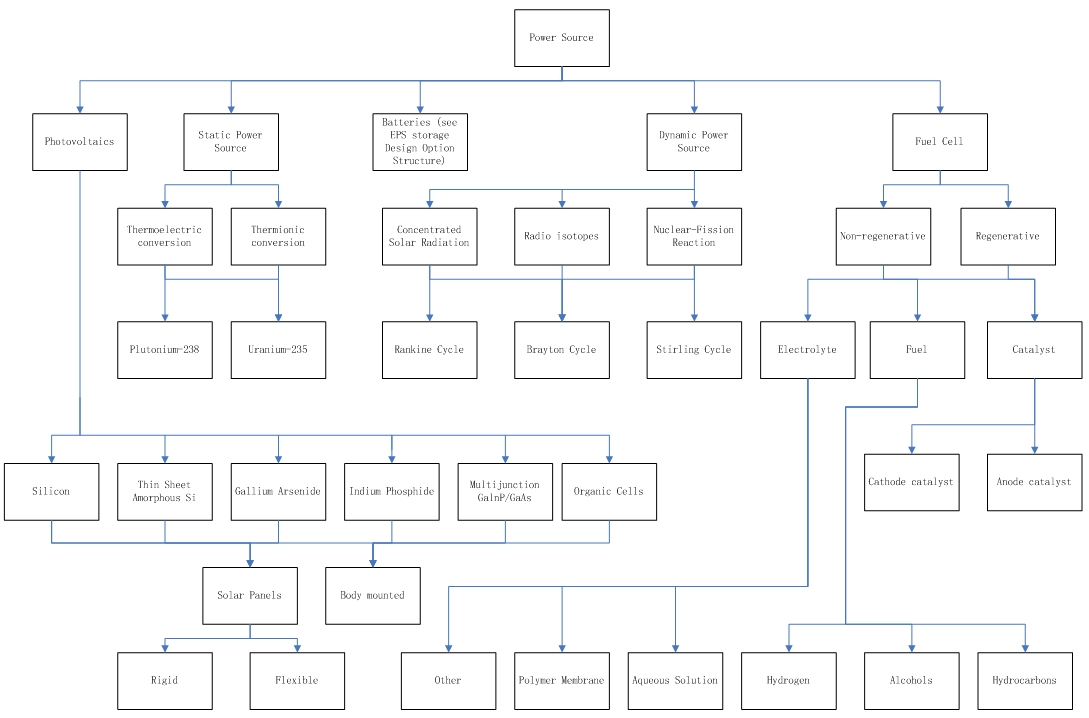
\includegraphics[width=1.0\textwidth, angle=90]{chapters/img/DOTeps_source.jpg}
\caption{Design option tree for the power source}
\label{pic_DOTeps_source}
\end{figure}

\begin{figure}
\centering
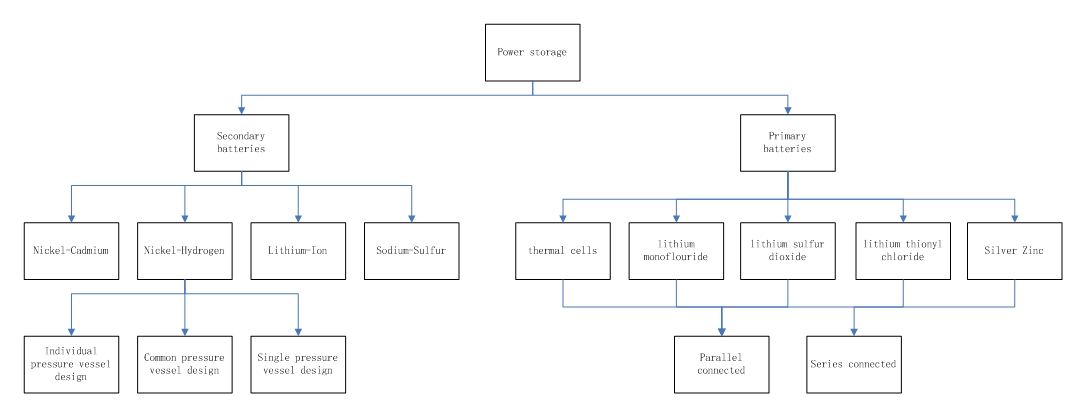
\includegraphics[width=1.0\textwidth, angle=90]{chapters/img/DOTeps_storage.jpg}
\caption{Design option tree for the power storage}
\label{pic_DOTeps_storage}
\end{figure}

\begin{figure}
\centering
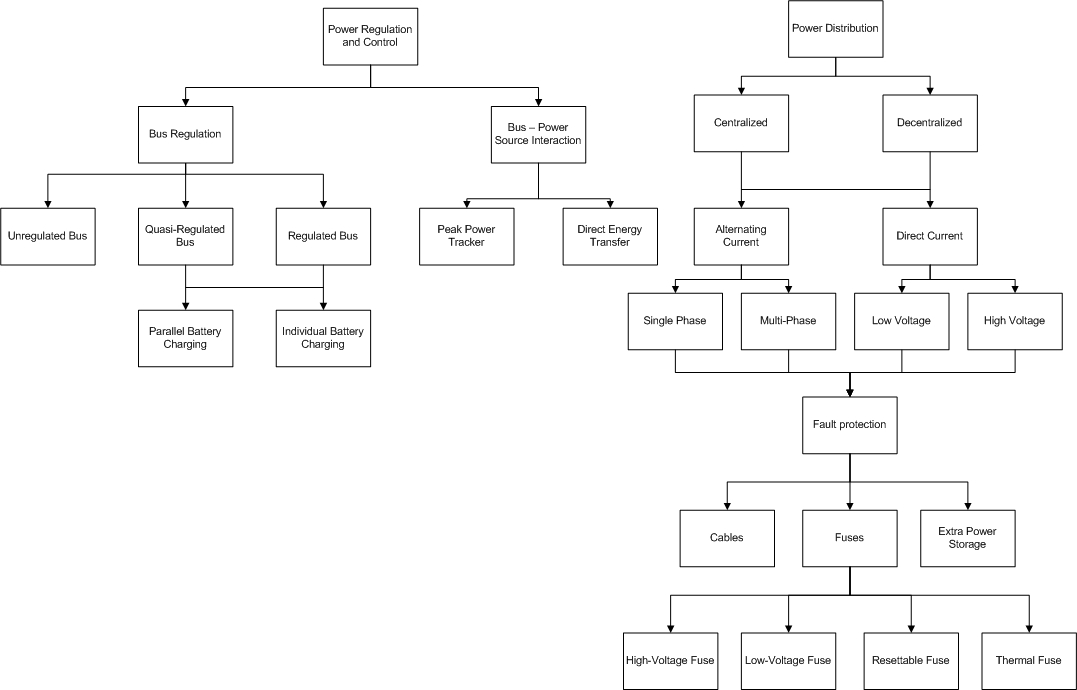
\includegraphics[width=1.0\textwidth, angle=90]{chapters/img/DOTeps_reganddis.jpg}
\caption{Design option tree for the distribution and regulation and control of the EPS}
\label{pic_DOTeps_reganddis}
\end{figure}